\begin{chaptercover}{Scope}%
{\coverepigraph{``Drones cause problems for more and more types of secure sites, whether it’s a matter of irresponsible or nefarious operators […] taking photos where you shouldn’t be taking photos or putting people on the ground at risk."}{\textsc{Nimo Shkedy} \newline {\normalsize\vspace{-.3cm}CEO of ApolloShield}}
{\large \hyphenation{} \bigletter{}{} {\color{red} ...}\newline\\}}%
{scope}

Now that we have set the basics of what is penetration testing, we can move to the actual application of the concept to the drones. 

The first phase of the work consists in gathering as much information as possible regarding the current state-of-the-art on drone security.

\section{Literature review}

This section focuses on showing a possible design of a drone and a compilation of security-relevant information. As part of that effort, the following emphasizes on giving a ready reference of one particular vulnerable drone and associated open source attack tools that have already been developed. This compilation should provide the reader with a better understanding of how drone vulnerability is currently exploited, and how future drone will take advantage of improvements in available vulnerability research data.

\subsection{Typical drone design}



\subsection{Parrot AR Drone}

\begin{center}
\begin{tabular}{m{5cm}m{12.3cm}}
\hyphenation{produced}
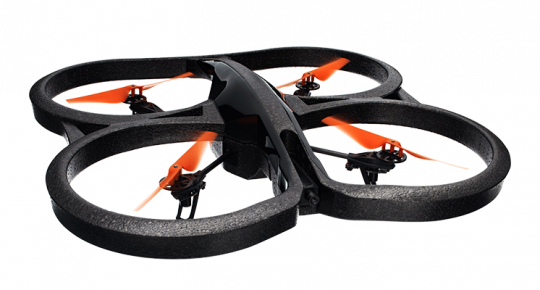
\includegraphics[width=\linewidth]{parrot-ar-drone-2} & The Parrot AR Drone 2.0 is one of the most popular quadcopters produced. This is a cheap drone that is both quick and fast. It is controlled by an iOS or Android smartphone or tablet and allows 720p live high-definition video streaming and recording in flight. \\
\end{tabular}
\end{center}

This device is a good reference on how one of the most popular commercial drones totally lacks security. Security breaches are numerous, let’s review them :
\begin{itemize}
  \item \textbf{Open FTP on port TCP/21} : Simply just connect to the IP without any username or password, and have access to the directory of the drone, where it stores the recorded videos.
  \item \textbf{Open Telnet on port 23} : Once again, simply just connect to the IP without any username or password, and you are logged in. Furthermore, it's running Linux and it is a root access to the device! At this point the attacker could simply issue a shutdown and watch the drone fall to the ground.
  \item \textbf{Unencrypted communications} : A simple capture of the communication packets between the drone and the controller allows the attacker to have an easy view of the protocol. Once he has successfully analyzed the main commands, he can easily replay them -- for example using the python Scapy library -- in order to hijack the drone.
  \item \textbf{WiFi controlled} : The drone is controlled with an app through WiFi, and by default, it isn’t even password-protected ! This allows any user running the application to control the drone. Even though a security can be enabled, called \textit{Pairing}, which will make the drone drop the packets if the MAC address sending them is not the one it is paired with. It is nonetheless easy for the attacker to spoof the source MAC on the packets.
\end{itemize}

More information can be found on the subject at \cite{github-drone-hacking} as well as some investigations for improving the security at \cite{hacking-securing-ardrone2}.

\subsection{Known vulnerabilities}

As defined in Subsection \ref{subsec:vuln-vs-weakness}, \acrshort{cve}'s are identifiers for publicly known vulnerabilities. It is therefore useful, prior to starting any pentest on drones, to look for eventual known vulnerabilities on the field. In the same way, CVE may be used once a certain service is identified on a device.

As for now, only one entry is available and concerns the DBPOWER U818A WIFI quadcopter drone :
\begin{itemize}
  \item \textbf{CVE-2017-3209} : \textit{The quadcopter drone provides \textbf{FTP} access over its own local access point, and allows full file permissions to the anonymous user. The DBPower U818A WIFI quadcopter drone runs an FTP server that by default \textbf{allows anonymous access without a password}, and provides full filesystem read/write permissions to the anonymous user. A remote user within range of the open access point on the drone may utilize the anonymous user of the FTP server to read arbitrary files, such as images and video recorded by the device, or to replace system files such as /etc/shadow to gain further access to the device. Furthermore, the DBPOWER U818A WIFI quadcopter drone uses BusyBox 1.20.2, which was released in 2012, and may be vulnerable to other known BusyBox vulnerabilities.}
\end{itemize}

It goes without saying that a single result is terribly weak, for example, we get nearly 1,500 results just for the Apache web server (as August 2019). This tends to show that a substantive work remains to be done in this area, but also that the door is open for real progress.

{\color{red}
Here insert a note on some commercial projects such as:
\begin{itemize}
  \item ApolloShield:  https://www.apolloshield.com/
  \item Talk about the many “non-hacking” solutions
\end{itemize}}

\section{Scope definition}

This section presents some models of drones selected for the study and the beginning of the application of the penetration testing methodology, that is, the \textit{intelligence gathering}.

\subsection{Scope limitation}

The drones were provided by the professional supervisor within the limits of his allocated budget to cover a small spectrum of drone-related technologies in order to establish the basis of a framework (as it is explained in Chapter \ref{framework}). For a question of scope, only a few models are selected to match some technical specifications as we focus on wireless penetration testing.

For this work, we received the following six different drones. Each of them comes from a different brand so that we can cover the wider spectrum of technologies possible.
\begin{itemize}
  \item Drone S9
  \item Jamara Skip 3D Quadrocopter
  \item NINCOAIR QUADRONE MINI
  \item UdiR/C Free Loop U27 
  \item Flitt Selfie Cam
  \item C-me 1080P WiFi FPV GPS Selfie Drone
\end{itemize}

In the initial problem statement, it was decided to develop plugins for at least 3 different popular commercial drones on the framework according to the exploits that could be discovered. Rather quickly, we excluded the first four since they were not WiFi- but radio-controlled and should require the use of a different technology than the one aimed in this work. It leaved us with the last two.

\subsection{Flitt Selfie Cam}

\begin{center}
\begin{tabular}{m{5cm}m{12.3cm}}
\hyphenation{produced}
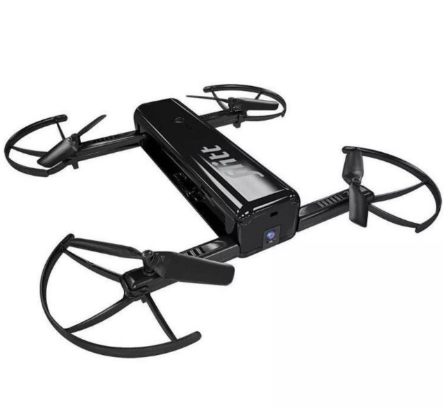
\includegraphics[width=\linewidth]{figures/flitt-selfie-cam} & \textit{Flitt Flying Camera is a pocket-sized flyer that features an adjustable CMOS camera that can record 720p video at 30 fps and shoot 1.3MP photos. The Flitt uses 2.4 GHz Wi-Fi to communicate with either an Android or IOS free companion app. From the app, you can fly the Flitt, take pictures and video, adjust camera pitch, change the photo mode, and more.} \\
\end{tabular}
\end{center}

\begin{figure}[H]
  \centering
  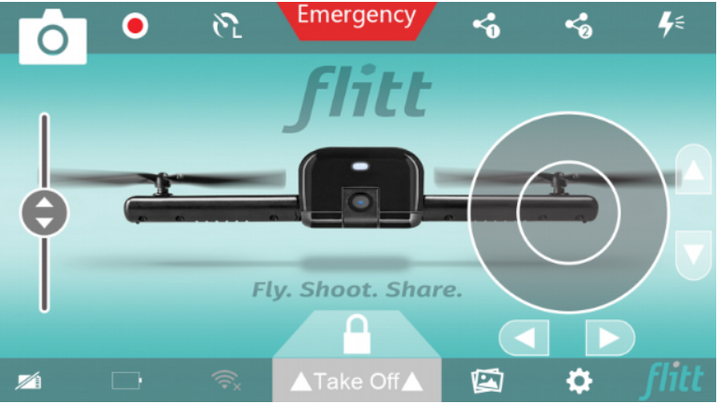
\includegraphics[width=0.7\linewidth]{figures/flitt-selfie-cam-ui}
  \caption{User interface for piloting the Flitt Selfie Cam from a smartphone}
  \label{fig:flitt-selfie-cam}
\end{figure}

The device must be unlocked in order to take off, auto-regulates its high and has an emergency landing feature in case of loss of control.

\subsection{C-me Selfie Drone}

\begin{center}
\begin{tabular}{m{5cm}m{12.3cm}}
\hyphenation{produced}
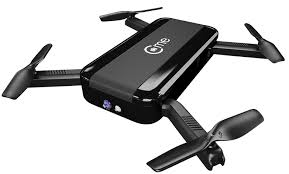
\includegraphics[width=\linewidth]{figures/cme-selfie-drone} & \textit{C-me flying camera is designed to be the ultimate flying "selfie stick" for capturing life’s memorable events thanks to its 8MP HD 1080p camera. It comes with an intuitive app control that interfaces with iOS and most Android phones and tablets. It communicates through 2.4 GHz Wi-Fi. Its size allows to easily fit in a pocket, purse or backpack.} \\
\end{tabular}
\end{center}

\begin{figure}[H]
  \centering
  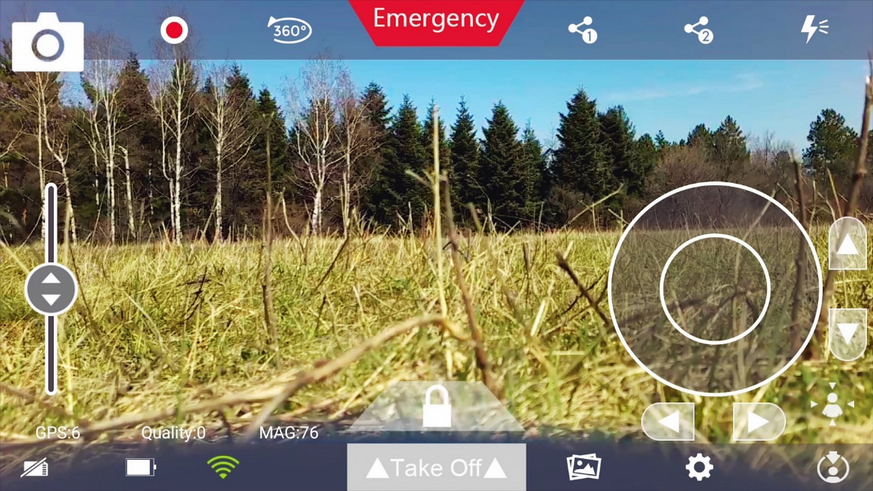
\includegraphics[width=0.7\linewidth]{figures/cme-selfie-drone-ui}
  \caption{User interface for piloting the C-me Selfie Drone from a smartphone}
  \label{fig:flitt-selfie-cam}
\end{figure}

Once again, the device must be unlocked in order to take off, auto-regulates its high and has an emergency landing feature in case of loss of control.

\begin{tip}
It is quite obvious that the interfaces are quite similar, and after further research, it turns out that the two drones are produced by the same manufacturer, i.e. Hobbico. This means that there will probably be similarities between the two devices, even though the C-me has more functionalities since it’s a little bit more expensive than the Flitt (depending on the reseller, in the 150\euro range versus 80\euro). This will be a good occasion to compare them and see if one is more secure than the other.

Hobbico, Inc. was a manufacturer and distributor of hobby products including radio control airplanes, boats, cars, helicopters and drones. Unfortunately, on 2018, it was announced that Hobbico had filed for Chapter 7 bankruptcy and went into liquidation1, and the company was later bought by Horizon Hobby2. There website, hobbico.com, is no longer available online and there is no reference to any of the drones on the Horizon Hobby website meaning that there is no support anymore for them.
\end{tip}

\subsection{Intelligence gathering}


\section{Vulnerability analysis}


\end{chaptercover}
